%% GENERATED by tools/from_docs.py from stepss-docs. Do not edit by hand:
%% edit the page named below in stepss-docs and regenerate.
%% source: stepss-docs/src/content/docs/models/injectors/compensation-measurement.md

\chapter{Compensation and measurement models}\label{doc:model-inj-comp}

Two injector models that are neither loads nor generators: a static var compensator and a phasor measurement unit.

The \texttt{INJEC} record these models are entered with, and the rules on model names, are on the Injector Models page.

\section{\texorpdfstring{SVC\_GENERIC1 (\texttt{inj\_svc\_generic1}): Generic Static Var Compensator}{SVC\_GENERIC1 (inj\_svc\_generic1): Generic Static Var Compensator}}\label{model-inj-comp:svc_generic1-inj_svc_generic1-generic-static-var-compensator}

The data-file model name is \texttt{SVC\_GENERIC1}. It takes no prefix.

\subsection{Description}\label{model-inj-comp:description}

A dynamic SVC injecting a purely reactive current at its bus. A PI voltage
regulator with droop drives a susceptance \(B_{svc}\) between \texttt{Bmin} and \texttt{Bmax},
and two lead-lag stabiliser channels can add a supplementary signal to the
voltage reference. This is the dynamic counterpart of the static
\hyperref[ch-pf]{SVC record} used by the
power flow: the static record fixes the operating point, this model governs how
the device behaves during the simulation.

The voltage reference is initialised from the power flow solution, so that the
model starts in equilibrium:

\[V_{ref} = V_0 + B_p \cdot B_{svc,0}\]

where \(B_p\) is the droop and \(B_{svc,0}\) the initial susceptance implied by the
reactive current at the bus.

\begin{figure}[htbp]
\centering
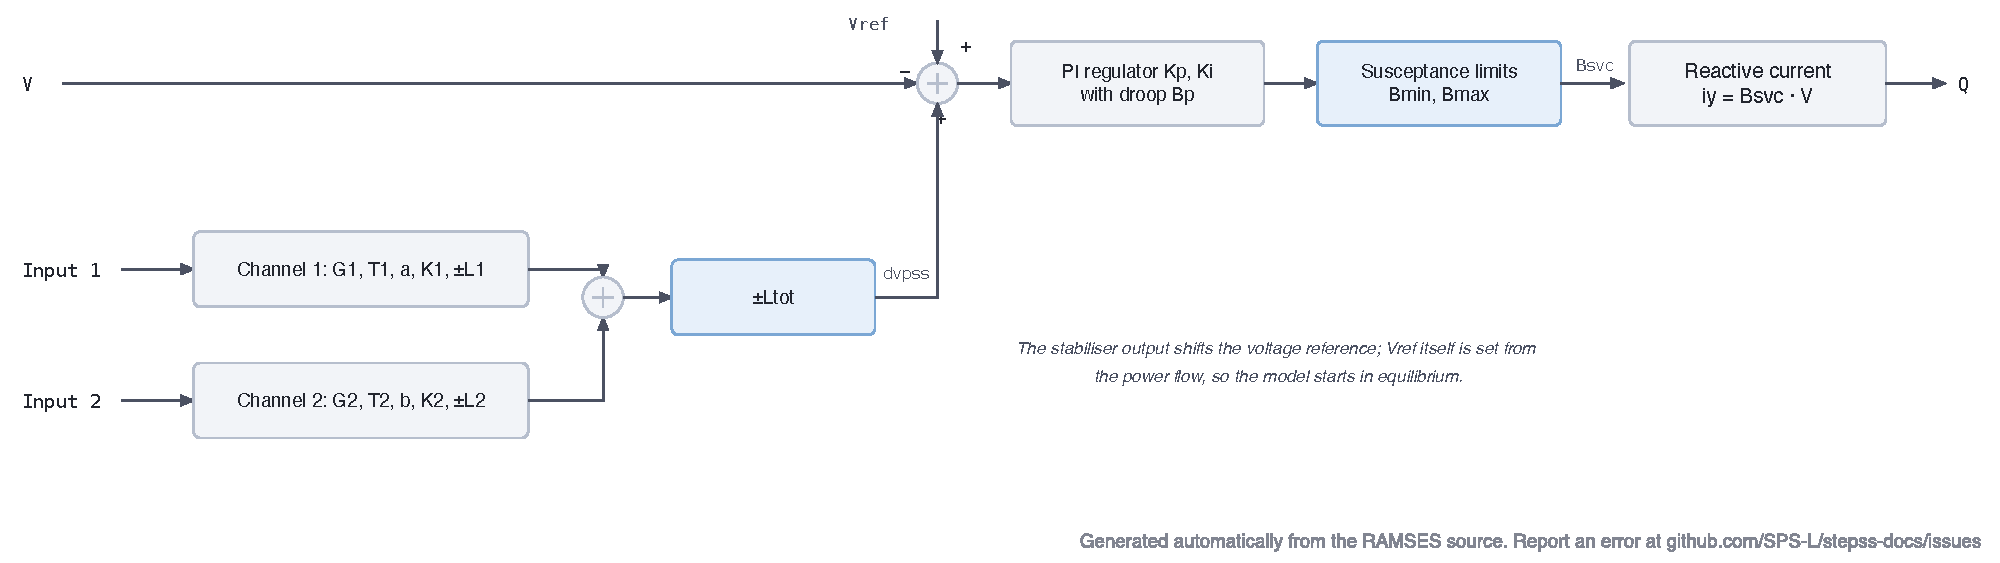
\includegraphics[width=0.98\linewidth]{figures/inj-svc-generic1-light}
\caption{Generic static var compensator block diagram.}
\end{figure}

\subsection{Parameters}\label{model-inj-comp:parameters}

The record carries 17 data parameters, in order:

\begin{small}\begin{longtable}[]{@{}
  >{\raggedright\arraybackslash}p{(\linewidth - 6\tabcolsep) * \real{0.1337}}
  >{\raggedright\arraybackslash}p{(\linewidth - 6\tabcolsep) * \real{0.1739}}
  >{\raggedright\arraybackslash}p{(\linewidth - 6\tabcolsep) * \real{0.6925}}
@{}}
\toprule\noalign{}
\begin{minipage}[b]{\linewidth}\raggedright
\#
\end{minipage} & \begin{minipage}[b]{\linewidth}\raggedright
Name
\end{minipage} & \begin{minipage}[b]{\linewidth}\raggedright
Description
\end{minipage} \\
\midrule\noalign{}
\endhead
\bottomrule\noalign{}
\endlastfoot
1 & \texttt{G1} & Gain of the first stabiliser channel \\
2 & \texttt{T1} & Time constant of the first stabiliser channel (s) \\
3 & \texttt{a} & Lead-lag coefficient of the first channel \\
4 & \texttt{K1} & Output gain of the first channel \\
5 & \texttt{L1} & Output limit of the first channel (pu) \\
6 & \texttt{G2} & Gain of the second stabiliser channel \\
7 & \texttt{T2} & Time constant of the second stabiliser channel (s) \\
8 & \texttt{b} & Lead-lag coefficient of the second channel \\
9 & \texttt{K2} & Output gain of the second channel \\
10 & \texttt{L2} & Output limit of the second channel (pu) \\
11 & \texttt{Ltot} & Limit on the summed stabiliser output (pu) \\
12 & \texttt{Kp} & Proportional gain of the voltage regulator \\
13 & \texttt{Ki} & Integral gain of the voltage regulator \\
14 & \texttt{Bp} & Droop, in pu on the SVC base \\
15 & \texttt{Bmax} & Maximum susceptance (Mvar at 1 pu voltage) \\
16 & \texttt{Bmin} & Minimum susceptance (Mvar at 1 pu voltage) \\
17 & \texttt{Bnom} & Susceptance base used for the per-unit conversion (Mvar) \\
\end{longtable}\end{small}

One additional parameter is computed at initialisation:

\begin{small}\begin{longtable}[]{@{}lll@{}}
\toprule\noalign{}
\# & Name & Description \\
\midrule\noalign{}
\endhead
\bottomrule\noalign{}
\endlastfoot
18 & \texttt{Vref} & Voltage reference, set from the power flow solution \\
\end{longtable}\end{small}

\subsection{Observables}\label{model-inj-comp:observables}

\texttt{Q}, \texttt{dvpss}, \texttt{Bsvc}, \texttt{Vref}, \texttt{Vb}

\begin{center}\rule{0.5\linewidth}{0.5pt}\end{center}

\section{\texorpdfstring{PMU (\texttt{inj\_PMU}): Phasor Measurement Unit}{PMU (inj\_PMU): Phasor Measurement Unit}}\label{model-inj-comp:pmu-inj_pmu-phasor-measurement-unit}

The data-file model name is \texttt{PMU} (or \texttt{inj\_PMU}).

\subsection{Description}\label{model-inj-comp:description-1}

A measurement-only injector: it injects \textbf{zero current} at its bus and exists
purely to expose bus quantities as observables. It reports a filtered local
frequency estimate computed the same way as the \texttt{f\_inj} block, together with the
bus voltage magnitude and angle and the speed and angle of the moving DQ
reference frame. Attach one to any bus whose frequency you want to record
without perturbing the solution.

The frequency estimate is a first-order filter on the bus voltage phasor. The
measurement time constant is clamped to a floor of 0.05 s, so values below that
have no effect.

\begin{figure}[htbp]
\centering
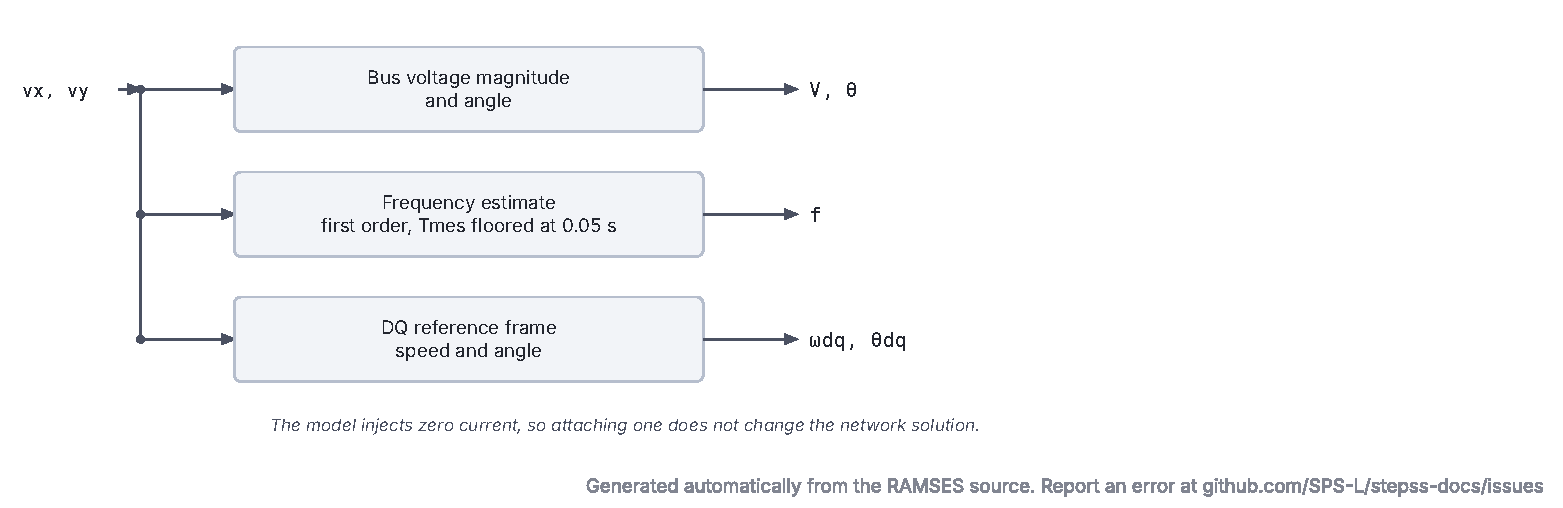
\includegraphics[width=0.98\linewidth]{figures/inj-pmu-light}
\caption{Phasor measurement unit block diagram.}
\end{figure}

\subsection{Parameters}\label{model-inj-comp:parameters-1}

\begin{small}\begin{longtable}[]{@{}
  >{\raggedright\arraybackslash}p{(\linewidth - 8\tabcolsep) * \real{0.0870}}
  >{\raggedright\arraybackslash}p{(\linewidth - 8\tabcolsep) * \real{0.1508}}
  >{\raggedright\arraybackslash}p{(\linewidth - 8\tabcolsep) * \real{0.6246}}
  >{\raggedright\arraybackslash}p{(\linewidth - 8\tabcolsep) * \real{0.1376}}
@{}}
\toprule\noalign{}
\begin{minipage}[b]{\linewidth}\raggedright
\#
\end{minipage} & \begin{minipage}[b]{\linewidth}\raggedright
Name
\end{minipage} & \begin{minipage}[b]{\linewidth}\raggedright
Description
\end{minipage} & \begin{minipage}[b]{\linewidth}\raggedright
Unit
\end{minipage} \\
\midrule\noalign{}
\endhead
\bottomrule\noalign{}
\endlastfoot
1 & \texttt{Tf} & Frequency measurement time constant, recommended 0.05 to 0.10; values below 0.05 are clamped & s \\
\end{longtable}\end{small}

Three additional parameters are set at initialisation: \texttt{wnom} (nominal angular
frequency), \texttt{vm0} and \texttt{va0} (the initial bus voltage magnitude and angle).

\subsection{Observables}\label{model-inj-comp:observables-1}

\begin{small}\begin{longtable}[]{@{}
  >{\raggedright\arraybackslash}p{(\linewidth - 6\tabcolsep) * \real{0.1648}}
  >{\raggedright\arraybackslash}p{(\linewidth - 6\tabcolsep) * \real{0.6281}}
  >{\raggedright\arraybackslash}p{(\linewidth - 6\tabcolsep) * \real{0.2071}}
@{}}
\toprule\noalign{}
\begin{minipage}[b]{\linewidth}\raggedright
Name
\end{minipage} & \begin{minipage}[b]{\linewidth}\raggedright
Description
\end{minipage} & \begin{minipage}[b]{\linewidth}\raggedright
Unit
\end{minipage} \\
\midrule\noalign{}
\endhead
\bottomrule\noalign{}
\endlastfoot
\texttt{f} & Estimated bus frequency & pu of \(f_{nom}\) \\
\texttt{vm} & Bus voltage magnitude & pu \\
\texttt{va} & Bus voltage phase angle in the moving DQ frame, wrapping at \(\pm\pi\) & rad \\
\texttt{thref} & Accumulated angle of the DQ reference frame with respect to the nominally rotating frame, zero at \(t = 0\) & rad \\
\texttt{dwref} & Speed deviation of the DQ reference frame from nominal & rad/s \\
\end{longtable}\end{small}

\begin{docsnote}{Caution}

\texttt{dwref} and \texttt{thref} are only meaningful under \texttt{\$OMEGA\_REF\ COI}. With
\texttt{\$OMEGA\_REF\ SYN} the reference frame rotates at nominal speed by construction,
so both stay at zero.

\end{docsnote}

\subsection{Usage Example}\label{model-inj-comp:usage-example}

\begin{Verbatim}
INJEC  PMU  PMU_1041  1041
      # FP FQ P Q: share of the power-flow injection (FP, FQ) or initial power (P in MW, Q in Mvar)
      0.  0.  0.  0.
      # Tf: Frequency measurement time constant, recommended 0.05 to 0.10; values below 0.05 are clamped (s)
      0.05
;
\end{Verbatim}

All four participation and power fields are zero: the model neither consumes nor
produces power.
